\chapter{Dise\~no e implementaci\'on}\label{CAP:Disenoimplementacion}
En este cap\'itulo se comentar\'an los aspectos m\'as relevantes del dise\~no e implementaci\'on del sistema realizado, siendo la parte central de esta memoria.\\ 

\section{Introducci\'on}
En ingenier\'ia del software el t\'ermino fases del desarrollo expresa c\'omo ha progresado el desarrollo de un software y cu\'anto desarrollo ha sido requerido. Cada versi\'on importante de un producto pasa generalmente a trav\'es de una etapa en la que se agregan las nuevas caracter\'isticas (etapa alfa), despu\'es una etapa donde se eliminan errores activamente (etapa beta), y finalmente una etapa donde se han quitado todos los \textit{bugs} \footnote[1]{\textit{Bug} es un error de software que desencadena un resultado indeseado.} importantes (etapa estable). Las etapas intermedias pueden tambi\'en ser reconocidas.\\

Las etapas se pueden anunciar y regular formalmente por los desarrolladores del producto, pero los t\'erminos se utilizan a veces de manera informal para describir el estado de un producto. Normalmente muchas compa\~n\'ias usan nombres en clave para las versiones antes del lanzamiento de un producto, aunque el producto y las caracter\'isticas reales son raramente secretas.\\

\begin{figure}[htbp]
	
	\centering
	
\includegraphics[scale=0.5]{./Figuras/ingenieriadelsw.jpg}
	\caption{Ingenier\'ia del \textit{Software}.}
	\label{fig:ingSW}
	
\end{figure}

Para comenzar un proyecto en ingenier\'ia de software, debemos saber de manera clara qu\'e necesidades se pretenden cubrir con el resultado final. De igual modo, para el desarrollo de este tipo de proyectos se realizan una serie de tareas entre la idea inicial y el producto final. Ese desarrollo sigue una determinada metodolog\'ia o modelo de desarrollo, el cual establece el orden en el que se llevan a cabo las tareas en el proyecto y provee de requisitos de entrada y salida para cada una de las actividades.\\

\section{Modelo de desarrollo}
En ingenier\'ia del software el desarrollo en cascada o modelo en cascada  \footnote[1] {Denominado as\'i por la posici\'on de las fases en el desarrollo de esta, que parecen caer en cascada \"por gravedad\" hacia las siguientes fases}, es el enfoque metodol\'ogico que ordena rigurosamente las etapas del proceso para el desarrollo de software, de tal forma que el inicio de cada etapa debe esperar a la finalizaci\'on de la etapa anterior. Al final de cada etapa, el modelo est\'a dise\~nado para llevar a cabo una revisi\'on final, que se encarga de determinar si el proyecto est\'a listo para avanzar a la siguiente fase. Este modelo fue el primero en originarse y es la base de todos los dem\'as modelos de ciclo de vida.\\

La versi\'on original fue propuesta por \textit{Winston W. Royce} en 1970 y posteriormente revisada por \textit{Barry Boehm} en 1980 e \textit{Ian Sommerville} en 1985. Un ejemplo de una metodolog\'ia de desarrollo en cascada es:

\begin{itemize}
	
\item An\'alisis de requisitos
\item Dise\~no del sistema
\item Dise\~no del programa
\item Codificaci\'on
\item Pruebas
\item Implantaci\'on
\item Mantenimiento

\end{itemize}

De esta forma, cualquier error de dise\~no detectado en la etapa de prueba conduce necesariamente al redise\~no y nueva programaci\'on del c\'odigo afectado, aumentando los costos del desarrollo. La palabra cascada sugiere, mediante la met\'afora de la fuerza de la gravedad, el esfuerzo necesario para introducir un cambio en las fases m\'as avanzadas de un proyecto. Si bien ha sido ampliamente criticado desde el \'ambito acad\'emico y la industria, sigue siendo el paradigma m\'as seguido a d\'ia de hoy.\\

Como ya se explic\'o en episodios anteriores, el fin de la aplicaci\'on web "TuErasmus", es la de una web colaborativa para alumnos de la ETSIT, y donde est\'e a su disposici\'on toda la informaci\'on necesaria de manera f\'acil, r\'apida y sencilla de todas las universidades que forman parte del programa Erasmus. Por tanto, comenzamos por estudiar y analizar qu\'e cosas hay que tener en cuenta para el desarrollo, y a definir los distintos m\'odulos que debemos implementar, dise\~nando cuidadosamente el sistema, tanto para la parte del servidor como para la parte del cliente.\\  

\section{Objetivos}
Para poder llevar a cabo el desarrollo de la aplicaci\'on, en primer lugar se deben definir una serie de objetivos que dar\'an nombre a los hitos que se ir\'an cumpliendo gradualmente para llegar al conjunto final.\\

\subsubsection{Conocimientos adquiridos}
Este proyecto puede tomarse como una manera de profundizar y adquirir conocimientos en las nuevas tecnolog\'ias de desarrollo de aplicaciones web. Dichas tecnolog\'ias son el presente y el futuro cercano del desarrollo web, por lo que tener una base s\'olida de cara a entrar en el mercado laboral resulta un objetivo primordial.\\

En primer lugar, quer\'ia obtener una experiencia mayor con el desarrollo web usando tecnolog\'ias vistas superficialmente en la carrera, as\'i como aprender e investigar sobre nuevas tecnolog\'ias. Una vez realizado el apartado de la documentaci\'on de todos los recursos que iba a usar me dediqu\'e a definir el dise\~no y p\'aginas que compond\'ian la aplicaci\'on web, \¿cu\'ales ser\'ian las p\'aginas p\'ublicas? \¿cu\'ales ser\'ian las p\'aginas privadas? \¿qu\'e tipo de informaci\'on se iba a gestionar? \¿a qu\'e tipo de usuarios estaba dirigida la aplicaci\'on web?\\

Con unas respuestas coherentes y razonables a todas las preguntas lanzadas comenc\'e a sumergirme en el mundo de la programaci\'on, de los m\'etodos, de las variables locales y globales... de todo aquello que te envuelve a la hora de programar.\\

\subsubsection{Requisitos}
El proyecto deb\'ia cumplir ciertos requisitos b\'asicos, que enumero a continuaci\'on.

\begin{itemize}
	\item \textbf{Usar las nuevas tecnolog\'ias HTML5, CSS3}: Tecnolog\'ias bastante integradas en el mundo laboral hoy en d\'ia, con lo que es un punto a favor el tener un manejo de ellas y el conocimiento suficiente para poder incluirlas en el trabajo del futuro.
	\item \textbf{Integrar JavaScript en la parte del usuario}: \textbf{Rapidez}, estando en el lado del cliente permite que muchas funciones del c\'odigo se ejecuten sin tener que contactar con el servidor y esperar una respuesta; \textbf{Simplicidad}, relativamente f\'acil de aprender y poner en pr\'actica; \textbf{Versatilidad}, juega muy bien con otros idiomas y se puede utilizar en una gran variedad de aplicaciones. Estar del lado del cliente reduce la demanda en el servidor.
	\item \textbf{Integrar la API de Google Maps}: Conjunto de API que permiten superponer datos propios sobre un mapa de Google Maps personalizado. Le da un atractivo a las aplicaciones web  y con la cobertura global m\'as precisa del mundo y una comunidad de mapas activa que incorpora actualizaciones diarias, los usuarios se beneficiar\'an de un servicio que mejora constantemente.
	\item \textbf{Gestionar de manera \'optima la informaci\'on de la aplicaci\'on}: Es el objetivo principal de la aplicaci\'on, jugar con informaci\'on de una manera divertida, din\'amica y donde poder interactuar con otros usuarios.
	\item \textbf{Ofrecer una experiencia de usuario atractiva y sencilla}: Con CSS3 y HTML5 se pretende dotar a la aplicaci\'on con una imagen actual, moderna, intuitiva y que permitiese un uso agradable.
\end{itemize}

\section{Etapas del desarrollo}
\subsection{Documentaci\'on}
Como primera etapa de desarrollo, como en cualquier proyecto, lo que se debe hacer para comenzar a trabajar en un proyecto es documentarse sobre las herramientas y tecnolog\'ias que se quieran usar. Esta etapa me llev\'o su tiempo, ya que muchas de las tecnolog\'ias usadas no las conoc\'ia en profundidad, por lo que tuve que hacer un estudio espec\'ifico de varios conceptos. Una vez revisada la documentaci\'on comenc\'e a definir el esqueleto de lo que ser\'ia mi aplicaci\'on web.\\

Previamente, se instalaron los frameworks de Django y Bootstrap para el apartado del dise\~no de la interfaz de usuario. Una vez instalados ambos entornos de desarrollo, Bootstrap se deb\'ia integrar en el proyecto Django para poder dar el estilo a las p\'aginas de la herramienta web.\\

\subsection{Dise\~no de la base de datos}
Ya funcionando los entornos, con sus configuraciones adecuadas, comenc\'e a trabajar con el pilar de la aplicaci\'on, \textbf{la base de datos}.\\

Quer\'ia que los usuarios a trav\'es de la aplicaci\'on fuesen capaces de registrarse, loguearse, cerrar sus sesiones, registrar perfiles de universidades, documentar las distintas universidade, acceder a los datos de los diversos usuarios... Ten\'ian que estar claramente definidas las tablas que formar\'ian dicha base de datos, para a posteriori poder hacer un buen uso de todos los datos que ofrecer\'ia la web.\\

Existen tres tablas con informaci\'on de los usuarios: \textit{Users}, \textit{UserProfile} y \textit{UsersUniversity}. Donde encontramos los datos m\'as importantes de los usuarios, nombre, correo electr\'onico, la universidad erasmus en la que estudi\'o...\\

En cuanto a las universidades encontramos un mayor n\'umero de tablas: \textit{University}, \textit{InfoBasic}, \textit{InfoGeneral}, \textit{InfoResidences}, \textit{InfoSubjects}, \textit{InfoCities}, \textit{Universities}. En estas tablas, encontramos la informaci\'on correspondietne a las residencias de cada universidad, la ciudad(con toda la informaci\'on relacionada) de una universidad, el conjunto de asignaturas de una universidad, los datos principales de cada una de las universidades, la informaci\'on espec\'ifica de la beca erasmus de una universidad.\\

Adem\'as de estas tablas, que son las m\'as importantes, existen otras que recogen datos gen\'ericos a las anteriormente enumeradas, y que optimizan la gesti\'on de datos.\\

\subsection{Creaci\'on del registro de usuarios}
\textbf{TuErasmus} iba tomando la forma de una comunidad de estudiantes erasmus. Por lo que esto implicaba un control de usuarios de la aplicaci\'on web. De este modo comienza a implementarse la parte del registro, login y logout de los miembros de la web.\\

\begin{figure}[htbp]
	
	\centering
	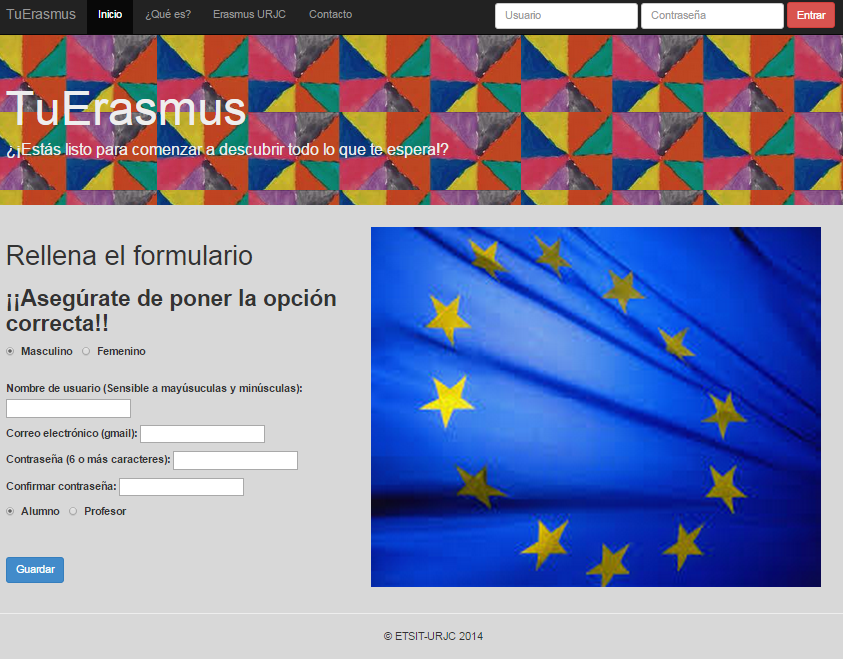
\includegraphics[scale=0.5]{./Figuras/tuerasmusPages/publicPages/register.png}
	\caption{Registro de usuarios}
	\label{fig:regUsu}
	
\end{figure}

En caso de introducir correctamente o err\'oneamente los datos en el formulario del registro nos aparecen unos mensajes indicando si hemos conseguido el registro de manera exitosa.\\

\begin{figure}[htbp]
	
	\centering
	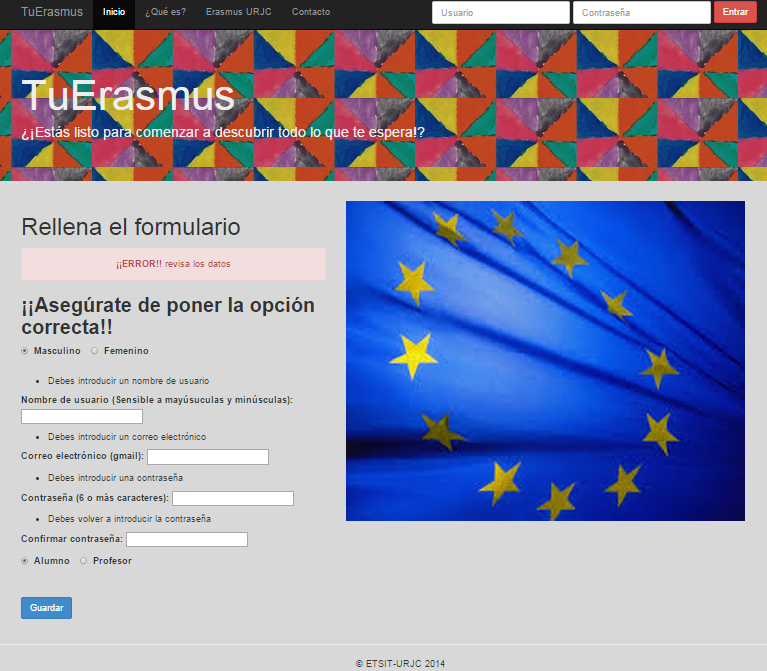
\includegraphics[scale=0.5]{./Figuras/tuerasmusPages/publicPages/errorRegister.png}
	\caption{Error registro de usuario}
	\label{fig:errRegUsu}
	
\end{figure}

\begin{figure}[htbp]
	
	\centering
	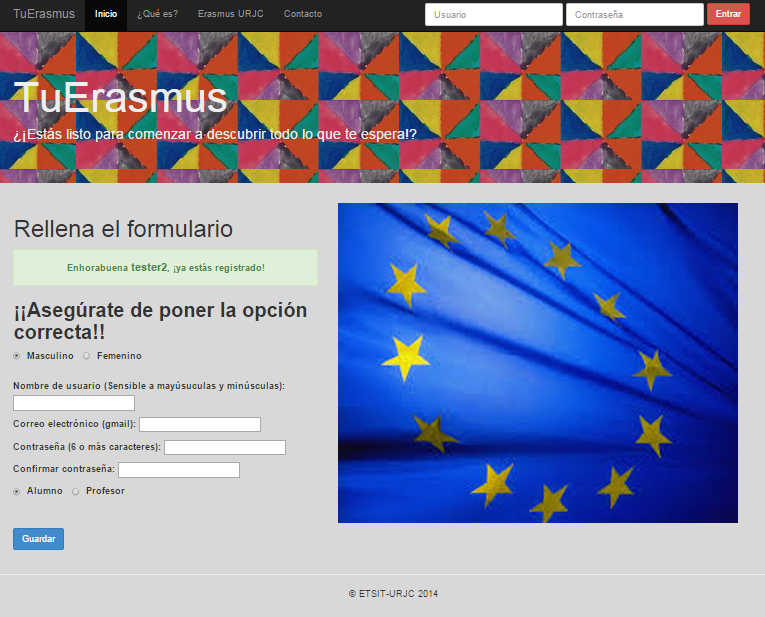
\includegraphics[scale=0.5]{./Figuras/tuerasmusPages/publicPages/successRegister.png}
	\caption{Exitoso registro de usuario}
	\label{fig:sucRegUsu}
	
\end{figure}

Los datos que se solicitan en este formulario son el nickname que tendr\'a ese usuario en la web, el correo electr\'onico para contactar en caso de ser necesario, si es alumno o profesor, ya que dependiendo de uno u otro, las asignaturas y comentarios ser\'an distintos, si eres chico o chica, sobre todo para la imagen que aparecer\'a en el perfil inicial del usuario por defecto. Estos datos por supuesto podr\'an ser modificados desde una de las interfaces de la aplicaci\'on donde se facilita un formulario permitiendo la modificaci\'on de los perfiles de usuario.\\

\begin{figure}[htbp]
	
	\centering
	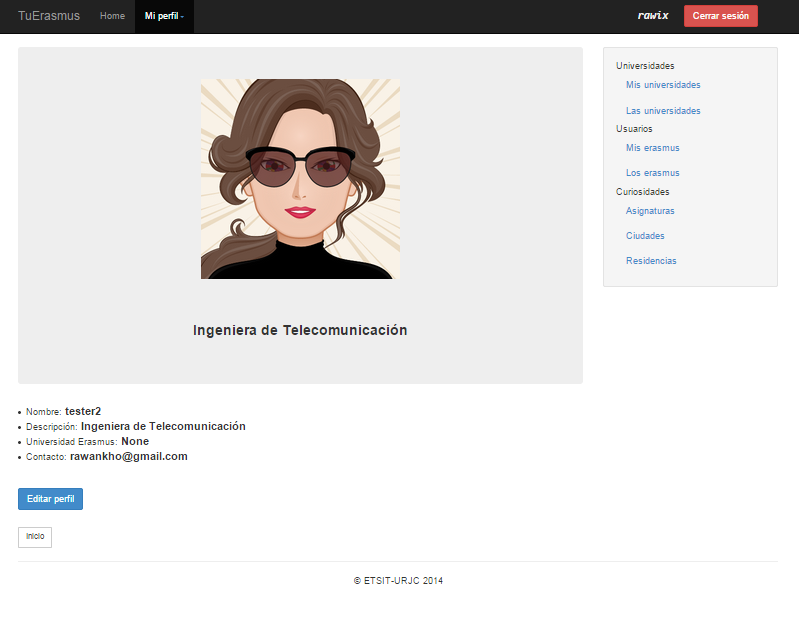
\includegraphics[scale=0.5]{./Figuras/tuerasmusPages/privatePages/myProfile.png}
	\caption{Mi perfil de usuario}
	\label{fig:profUsu}
	
\end{figure}

\begin{figure}[htbp]
	
	\centering
	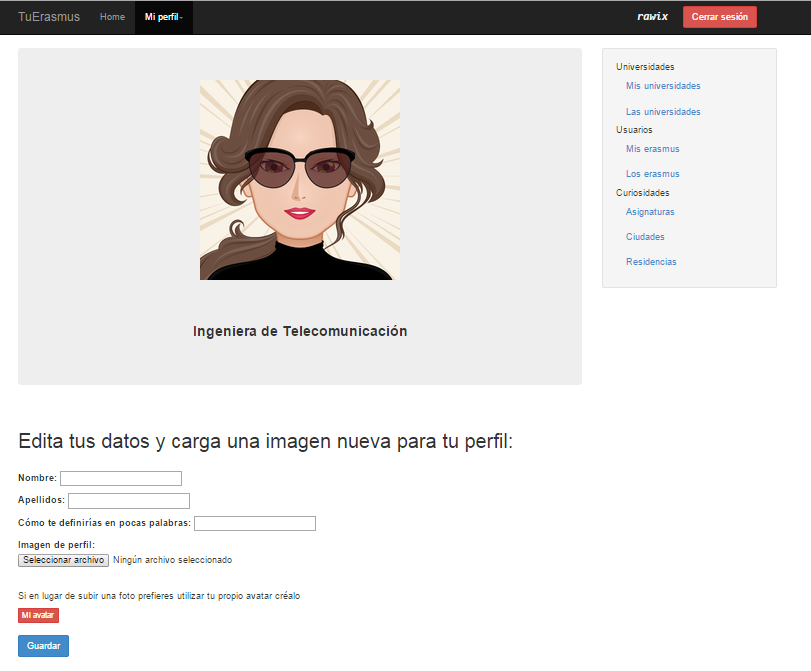
\includegraphics[scale=0.5]{./Figuras/tuerasmusPages/privatePages/editProfile.png}
	\caption{Editar mi perfil de usuario}
	\label{fig:editProfUsu}
	
\end{figure}

El hecho de tener que loguearse implica tener unos privilegios en cuanto al uso de la aplicaci\'on y a las ventajas de disponer de la informaci\'on acerca de las distintas universidades erasmus. Una vez logueados los usuarios, la navegaci\'on ser\'a por todo el conjunto de p\'aginas que forman la aplicaci\'on.\\

\subsection{Creaci\'on de perfiles de universidades}
Ya implementado el m\'etodo del registro de usuarios, me centr\'e en los m\'etodos correspondientes a la creaci\'on de los perfiles de cada universidad, as\'i como el dise\~no de los distintos formularios para los distintos temas a registrar en la base de datos.\\

\begin{figure}[htbp]
	
	\centering
	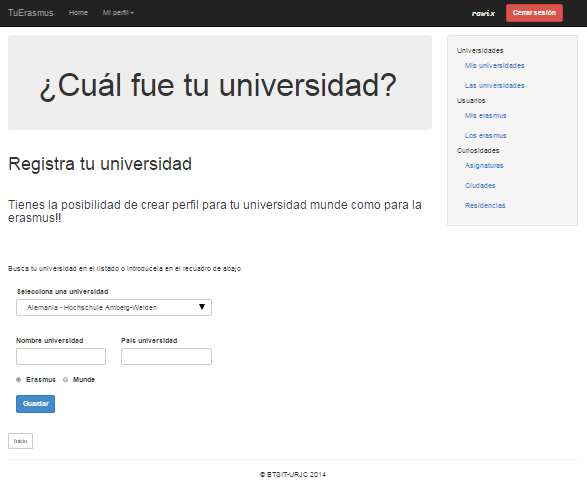
\includegraphics[scale=0.4]{./Figuras/tuerasmusPages/privatePages/uniRegister.png}
	\caption{Registro de universidades}
	\label{fig:uniReg}
	
\end{figure}

Al igual que con los perfiles de usuarios, los perfiles de las universidades tambi\'en son editables a elecci\'on del usuario, siempre y cuando sea de una manera constructiva para la comunidad erasmus (\textit{\nameref{fig:formBasic}}) y (\textit{\nameref{fig:formInfo}}).\\

\begin{figure}[htbp]
	
	\centering
	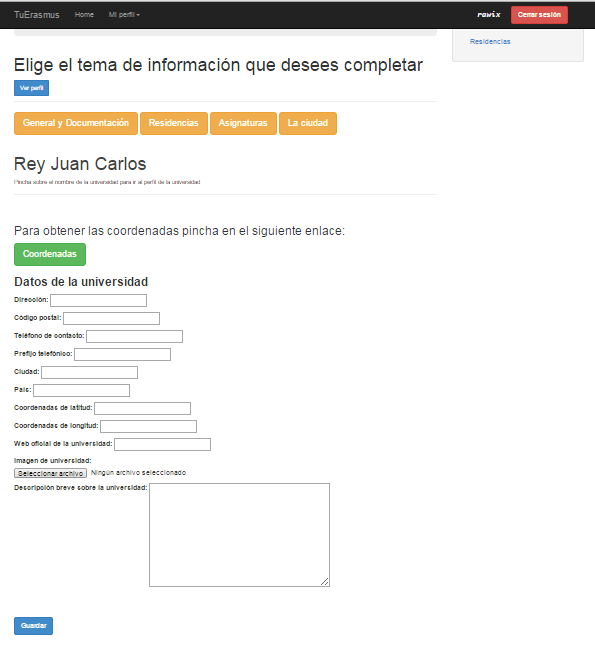
\includegraphics[scale=0.4]{./Figuras/tuerasmusPages/privatePages/formBasic.png}
	\caption{Formulario de los datos propios de la universidad}
	\label{fig:formBasic}
	
\end{figure}

\begin{figure}[htbp]
	
	\centering
	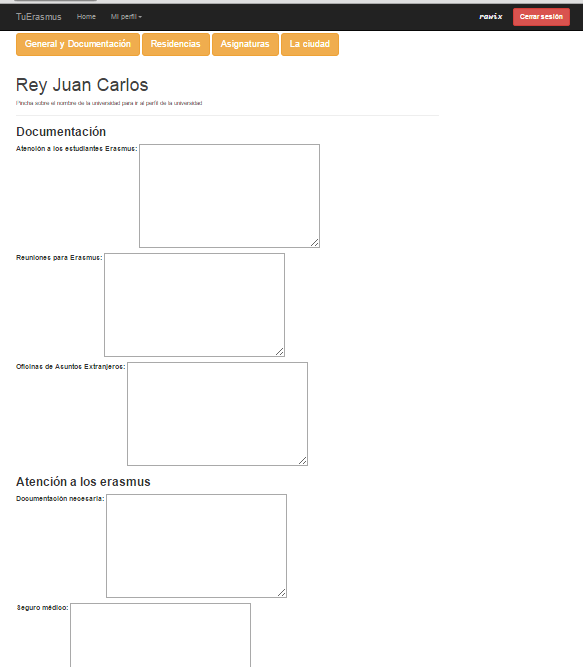
\includegraphics[scale=0.4]{./Figuras/tuerasmusPages/privatePages/formInfo.png}
	\caption{Formulario de la informaci\'on de la universidad}
	\label{fig:formInfo}
	
\end{figure}

\section{Arquitectura general}
La aplicaci\'on consta de una base de datos, donde se almacena toda la informaci\'on referente a la aplicaci\'on y diversas p\'aginas web. En primer lugar, cuando arrancamos la aplicaci\'on nos encontramos con la interfaz p\'ublica, cuya p\'agina inicial tiene una barra de navegaci\'on que nos permite navegar, como su propio nombre indica, por las distintas p\'aginas que forman la web \textbf{TuErasmus} e incluso poder iniciar sesi\'on.\\ 

\textit{\nameref{fig:navbar}}.\\
\begin{figure}[htbp]
	
	\centering
	
\includegraphics[scale=0.4]{./Figuras/tuerasmusPages/navbar.png}
	\caption{Barra de navegaci\'on}
	\label{fig:navbar}
	
\end{figure}

\textit{\nameref{fig:index}}, apreciamos un button en verde que nos redirige hacia la interfaz para el registro de usuarios a la web TuErasmus.\\
\begin{figure}[htbp]
	
	\centering
	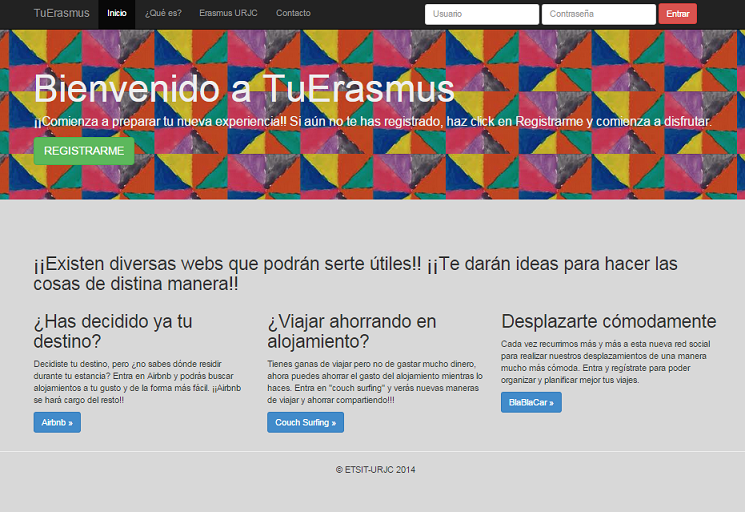
\includegraphics[scale=0.5]{./Figuras/tuerasmusPages/publicPages/index.png}
	\caption{P\'agina de inicio TuErasmus}
	\label{fig:index}
	
\end{figure}

\textit{\nameref{fig:howto}}.\\
\begin{figure}[htbp]
	
	\centering
	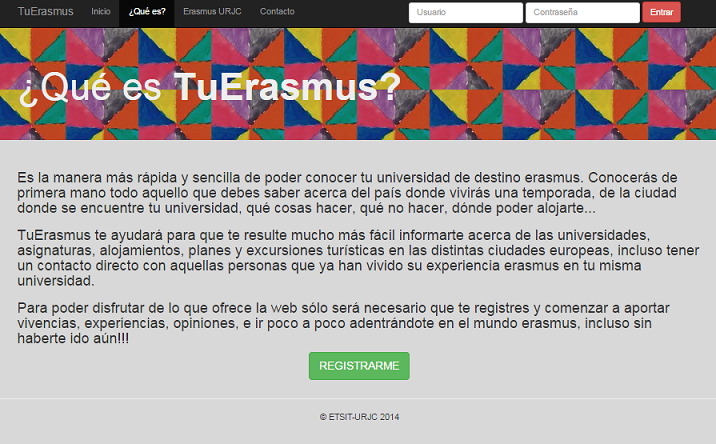
\includegraphics[scale=0.5]{./Figuras/tuerasmusPages/publicPages/howto.png}
	\caption{Breve descripci\'on de TuErasmus}
	\label{fig:howto}
	
\end{figure}

P\'agina a la que accedemos a trav\'es del link de la web de la urjc, donde se encuentra toda la informaci\'on correspondiente al programa erasmus (\textit{\nameref{fig:erasmusurjc}}).\\
\begin{figure}[htbp]
	
	\centering
	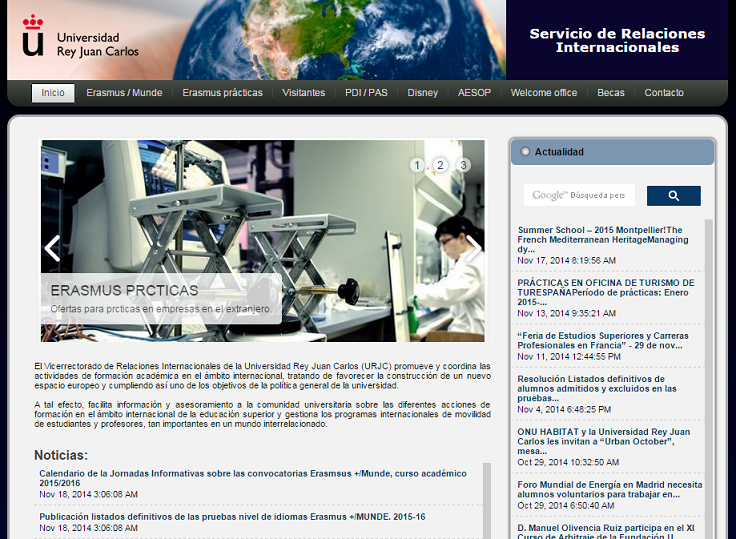
\includegraphics[scale=0.5]{./Figuras/tuerasmusPages/publicPages/erasmusurjc.png}
	\caption{Apartado de la web de la URJC dedicado al tema Erasmus}
	\label{fig:erasmusurjc}
	
\end{figure}

Una vez registrados y logueados, podremos navegar por las interfaces privadas de la web. Como p\'agina de inicio cuando estemos registrados encontramos una p\'agina donde observaremos una serie de pasos que guiar\'an al nuevo usuario para comenzar a ejecutar los primeros pasos, como registrar su universidad erasmus, comenzar a rellenar los distintos formularios sobre la ciudad, asignaturas, residencias, y dem\'as informaci\'on que nos puede resultar bastante \'util (\textit{\nameref{fig:home}}).\\

\begin{figure}[htbp]
	
	\centering
	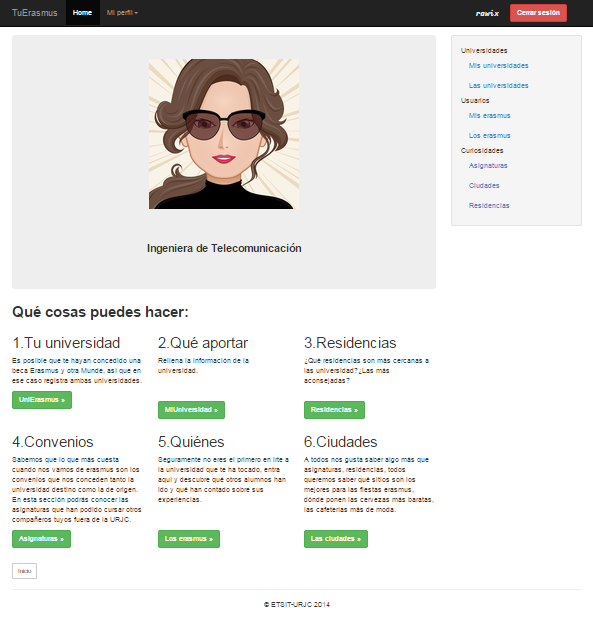
\includegraphics[scale=0.5]{./Figuras/tuerasmusPages/privatePages/home.png}
	\caption{P\'agina de home de la web TuErasmus}
	\label{fig:home}
	
\end{figure}

Tenemos varias maneras de navegar por la web, la primera es la barra de navegaci\'on de lo que es el navegador, desde donde podemos cerrar sesi\'on, ir a nuestro perfil y tambi\'en poder editarlo (\textit{\nameref{fig:navbarSup}}). En el lateral derecho tambi\'en disponemos de una columna de items desde donde podemos navegar en las distintas interfaces de la web, desde los perfiles de los usuarios hasta las distintas ciudades en las que han estado viviendo su experiencia erasmus (\textit{\nameref{fig:navbarDch}}). Y por \'ultimo cuando estemos en el perfil de una universidad tenemos una barra de navegaci\'on que nos permite navegar por los distintos temas documentados de cada universidad, como sus datos, asignaturas, residencias, la ciudad propia de esa universidad (\textit{\nameref{fig:navbarCen}}).\\

\begin{figure}[htbp]
	
	\centering
	
\includegraphics[scale=0.5]{./Figuras/tuerasmusPages/privatePages/navbarSup.png}
	\caption{Barra de navegaci\'on superior}
	\label{fig:navbarSup}
	
\end{figure}
\begin{figure}[htbp]
	
	\centering
	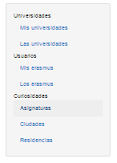
\includegraphics[scale=0.5]{./Figuras/tuerasmusPages/privatePages/navbarDch.png}
	\caption{Barra de navegaci\'on lateral derecho}
	\label{fig:navbarDch}
	
\end{figure}
\begin{figure}[htbp]
	
	\centering
	
\includegraphics[scale=0.7]{./Figuras/tuerasmusPages/privatePages/navbarCen.png}
	\caption{Barra de navegaci\'on con botones}
	\label{fig:navbarCen}
	
\end{figure}

\subsection{Navegaci\'on a trav\'es de los links del lateral derecho}
Las opciones de navegaci\'on de esta "barra de navegaci\'on" se corresponden con p\'aginas gen\'ericas sobre datos comunes de la web, es decir, que no encontraremos links directos a una secci\'on determinada de una unviersidad, si no que ser\'a el puente de acceso a los datos propios de una universidad.\\

Como links interesantes a mencionar encontramos el de \textit{misErasmus} (\textit{\nameref{fig:myEras}}) que recoge todos aquellos usuarios que est\'en registrados en nuestra misma universidad erasmus; \textit{losErasmus} (\textit{\nameref{fig:losEras}}) que recoge a todos los usuarios, agrupados por universidades; \textit{miUniversidad} (\textit{\nameref{fig:myUni}}) donde encontraremos un link directo al perfil de nuestra universidad (en la que pronto cursaremos nuestro programa erasmus o ya cursamos anteriormente el programa erasmus); \textit{lasUniversidades} (\textit{\nameref{fig:unis}}) donde veremos un listado de universidades, agrupadas por becas erasmus o becas mundus.\\

Como \'ultima secci\'on de esta parte lateral, tenemos tres enlaces que nos redirigen a una p\'agina de asignaturas gen\'ericas (\textit{\nameref{fig:asig}}), no espec\'ificas de una universidad, otro enlace a las diversas ciudades (\textit{\nameref{fig:ciud}}) de las universidades erasmus y por \'ultimo otro enlace a las residencias (\textit{\nameref{fig:res}}) de alumnos disponibles.\\

\begin{figure}[htbp]
	
	\centering
	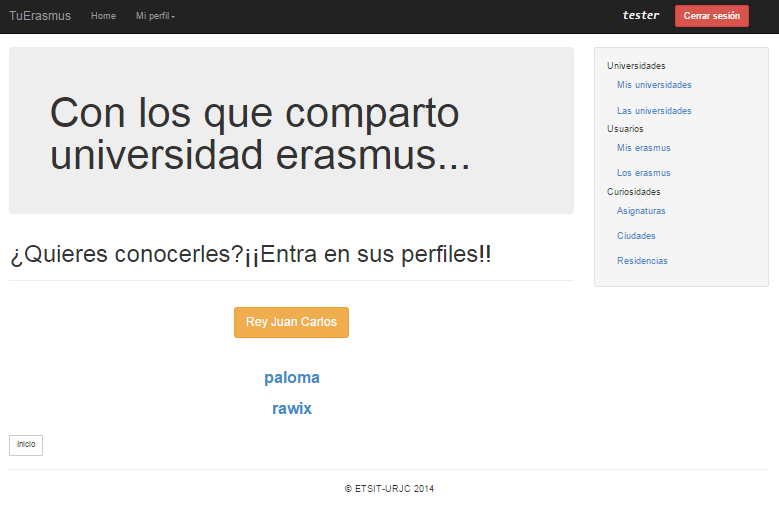
\includegraphics[scale=0.5]{./Figuras/tuerasmusPages/privatePages/myErasmus.png}
	\caption{P\'agina de mis erasmus}
	\label{fig:myEras}
	
\end{figure}
\begin{figure}[htbp]
	
	\centering
	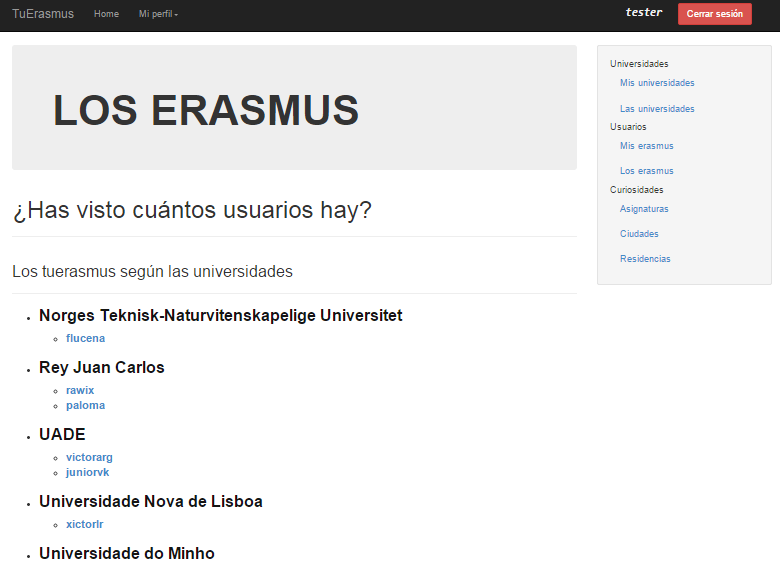
\includegraphics[scale=0.5]{./Figuras/tuerasmusPages/privatePages/losErasmus.png}
	\caption{P\'agina de los erasmus}
	\label{fig:losEras}
	
\end{figure}
\begin{figure}[htbp]
	
	\centering
	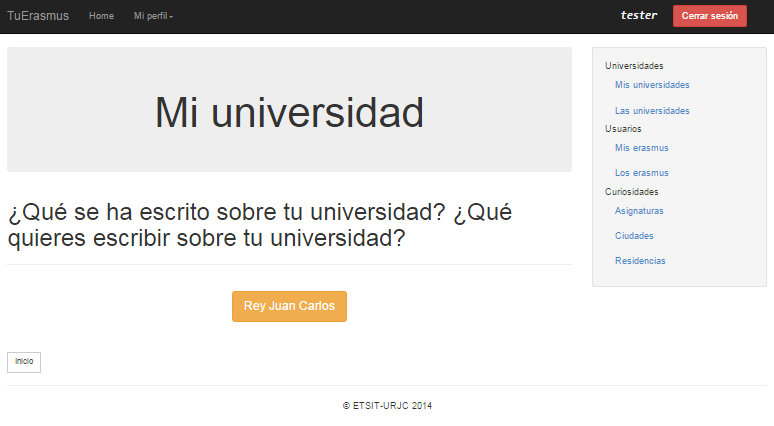
\includegraphics[scale=0.5]{./Figuras/tuerasmusPages/privatePages/myUniversity.png}
	\caption{Listado de universidades seg\'un el pa\'is}
	\label{fig:myUni}
	
\end{figure}
\begin{figure}[htbp]
	
	\centering
	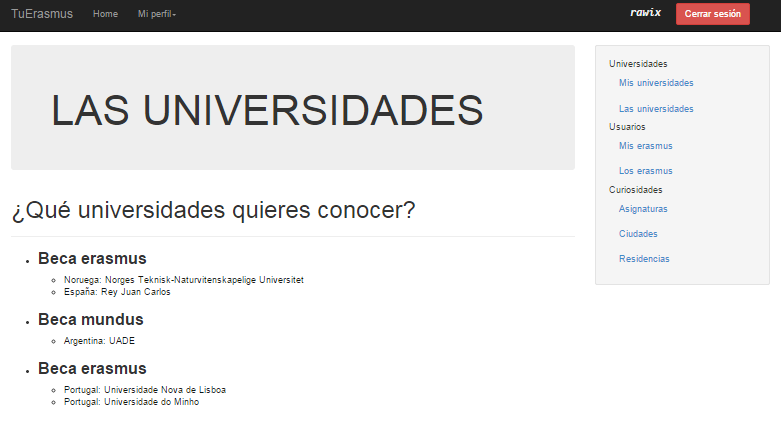
\includegraphics[scale=0.4]{./Figuras/tuerasmusPages/privatePages/universities.png}
	\caption{Listado de universidades seg\'un el programa}
	\label{fig:unis}
	
\end{figure}
\begin{figure}[htbp]
	
	\centering
	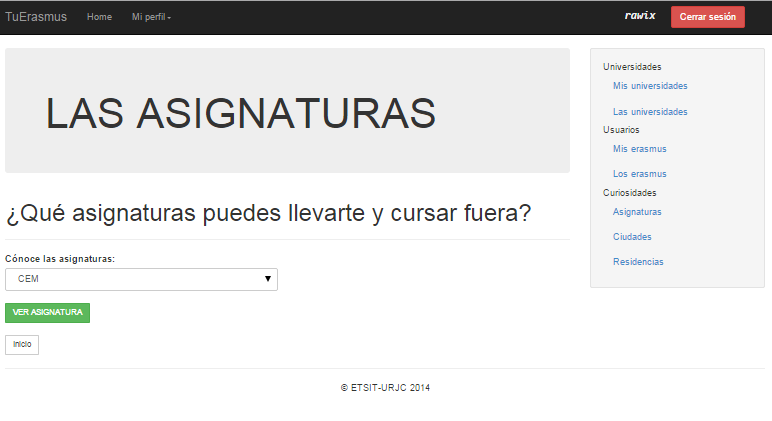
\includegraphics[scale=0.4]{./Figuras/tuerasmusPages/privatePages/asignaturas.png}
	\caption{P\'agina de las asignaturas}
	\label{fig:asig}
	
\end{figure}
\begin{figure}[htbp]
	
	\centering
	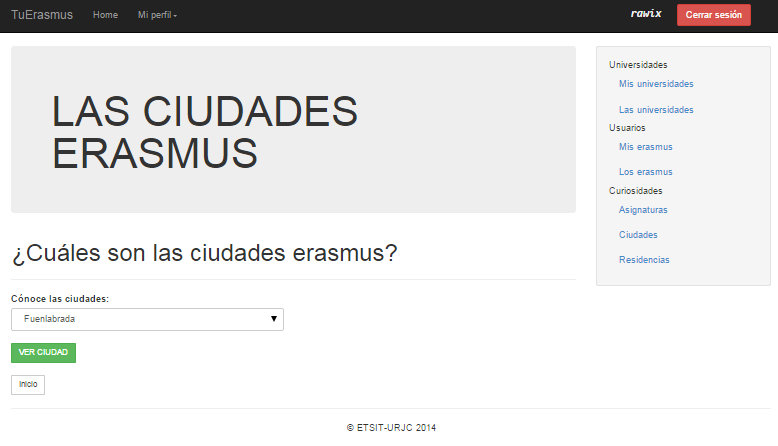
\includegraphics[scale=0.4]{./Figuras/tuerasmusPages/privatePages/ciudades.png}
	\caption{P\'agina de las ciudades erasmus}
	\label{fig:ciud}
	
\end{figure}
\begin{figure}[htbp]
	
	\centering
	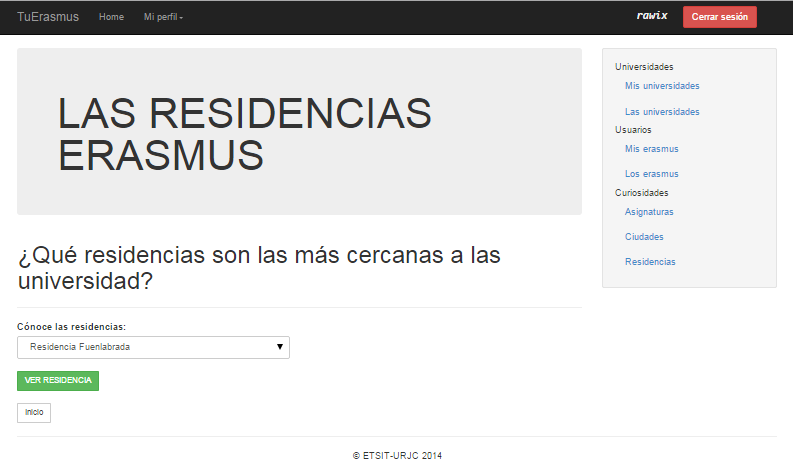
\includegraphics[scale=0.4]{./Figuras/tuerasmusPages/privatePages/residencias.png}
	\caption{P\'agina de las residencias}
	\label{fig:res}
	
\end{figure}

\subsection{Navegaci\'on por los botones de los perfiles de universidades}
En el perfil de cada universidad encontramos cinco botones cada uno correspondiente a un conjunto de informaci\'on. Por ellos podremos navegar por toda la informaci\'on propia de una unviersidad, y modificar y editar los perfiles, los comentarios de nuestro elemento principal, "la universidad".\\

En los perfiles (\textit{\nameref{fig:uniP}}), seg\'un la secci\'on en la que nos encontremos, la informaci\'on vendr\'a distribuida de diferente manera. En el caso de la p\'agina principal del perfil podemos observar un mapa con la localizaci\'on y los datos propios de esa universidad. Si estamos en las secciones de \textit{General} y \textit{Documentaci\'on} (\textit{\nameref{fig:uniI}}) encontramos la informaci\'on ordenada por puntos, con la opci\'on de poder modificar la documentaci\'on. En la secci\'on de las residencias (\textit{\nameref{fig:uniR}}) encontramos de nuevo un mapa con las localizaciones, y como \'ultimas secciones, tenemos las ciudades (\textit{\nameref{fig:uniC}}) y asignaturas (\textit{\nameref{fig:uniA}}) que tendr\'an un aspecto similar a las primeras secciones, y con las mismas posibilidades de modificar la informaci\'on.\\

\begin{figure}[htbp]
	
	\centering
	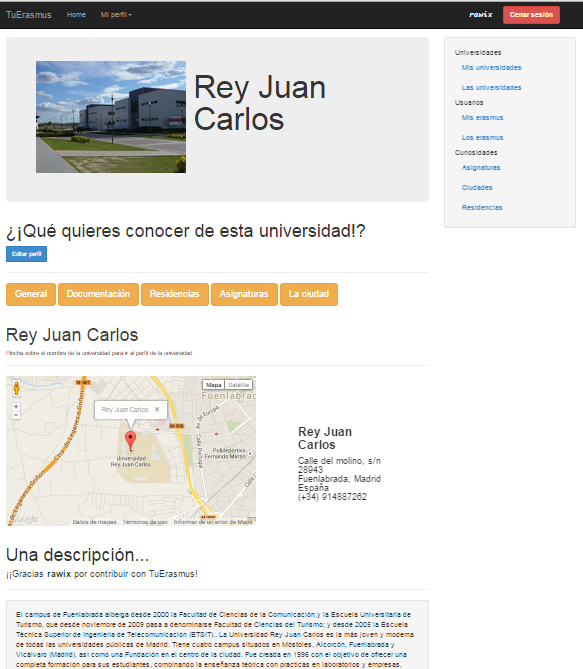
\includegraphics[scale=0.7]{./Figuras/tuerasmusPages/privatePages/uniProfile.png}
	\caption{Perfil de universidad}
	\label{fig:uniP}
	
\end{figure}
\begin{figure}[htbp]
	
	\centering
	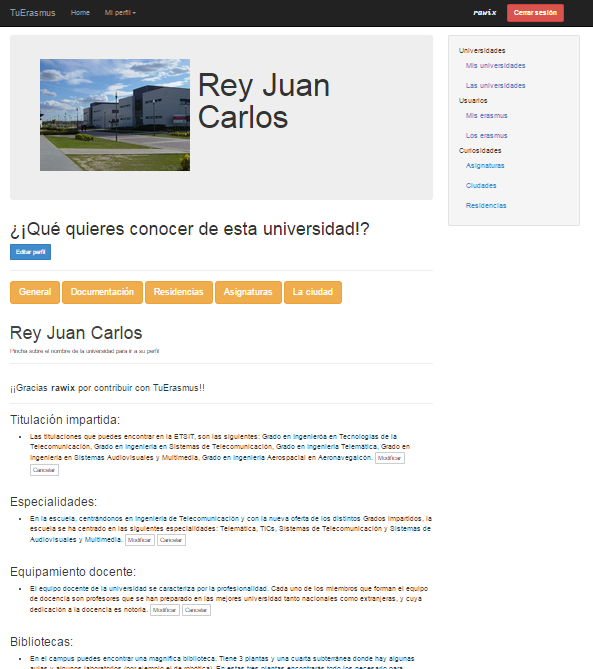
\includegraphics[scale=0.5]{./Figuras/tuerasmusPages/privatePages/uniInfo.png}
	\caption{P\'agina de la informaci\'on de la universidad}
	\label{fig:uniI}
	
\end{figure}
\begin{figure}[htbp]
	
	\centering
	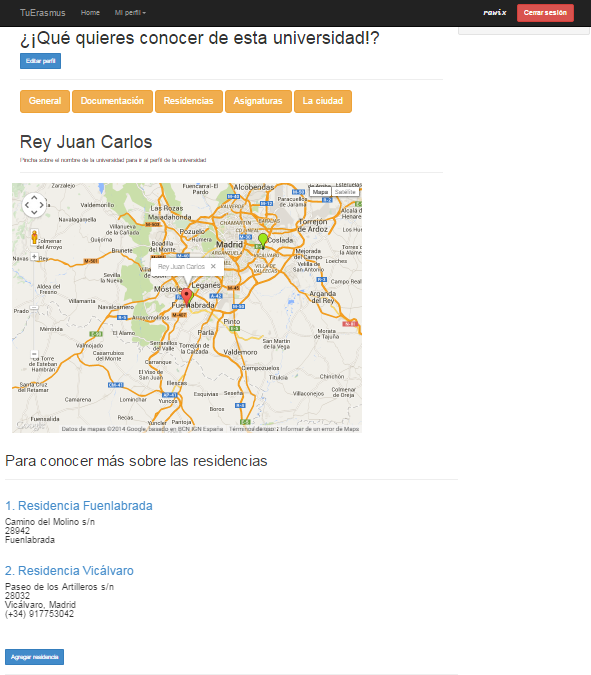
\includegraphics[scale=0.5]{./Figuras/tuerasmusPages/privatePages/uniResidencias.png}
	\caption{P\'agina de las residencias de la universidad}
	\label{fig:uniR}
	
\end{figure}
\begin{figure}[htbp]
	
	\centering
	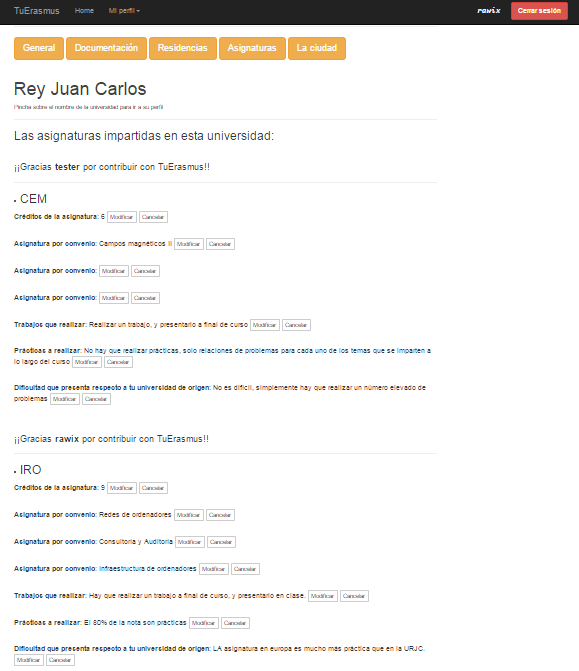
\includegraphics[scale=0.5]{./Figuras/tuerasmusPages/privatePages/uniAsignaturas.png}
	\caption{P\'agina de las asignaturas de la universidad}
	\label{fig:uniA}
	
\end{figure}
\begin{figure}[htbp]
	
	\centering
	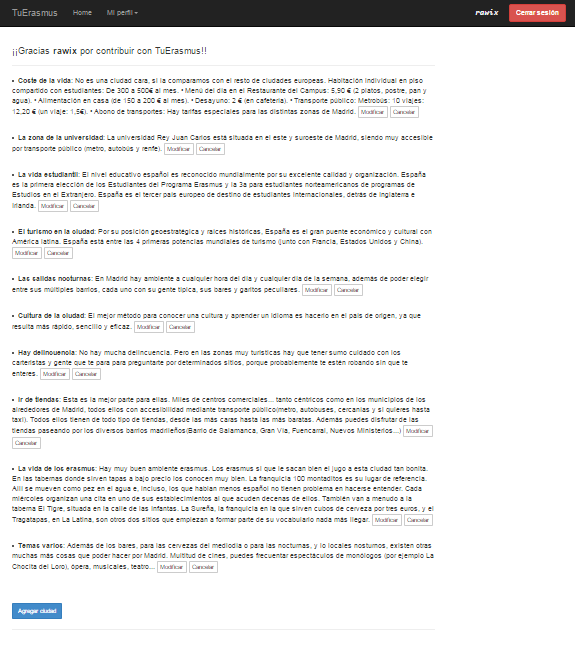
\includegraphics[scale=0.5]{./Figuras/tuerasmusPages/privatePages/uniCiudades.png}
	\caption{P\'agina de las ciudades de la universidad}
	\label{fig:uniC}
	
\end{figure}

\section{Conclusiones}
Tras este intenso cap\'itulo, agrada bastante ver el resultado final. Cuando comenc\'e a trabajar en este cap\'itulo me empezaron a venir a la mente todos aquellos momentos en los que me atasqu\'e y en los que no sab\'ia como avanzar. Pero investigando por mi cuenta, preguntando a personas con m\'as experiencia que yo y consultando a mi tutor consegu\'i salir exitosa de cualquier problema cr\'itico que he encontrado en el camino.\\

Desde luego, que los conceptos estudiados en la carrera los he afianzado much\'isimo con este maravilloso trabajo. He aprendido a organizar un proyecto para desarrollo de una aplicaci\'on web. Seguramente los errores que he cometido ahora no los cometer\'e en un futuro, no muy lejano.\\
